      \begin{figure*}
        \centering
        \begin{subfigure}[b]{0.34\textwidth}
            \centering
            \caption[]%
            {{\small Netpipe}}  
            \vspace*{-0.3cm}  
            \label{fig:perf_netpipe}
            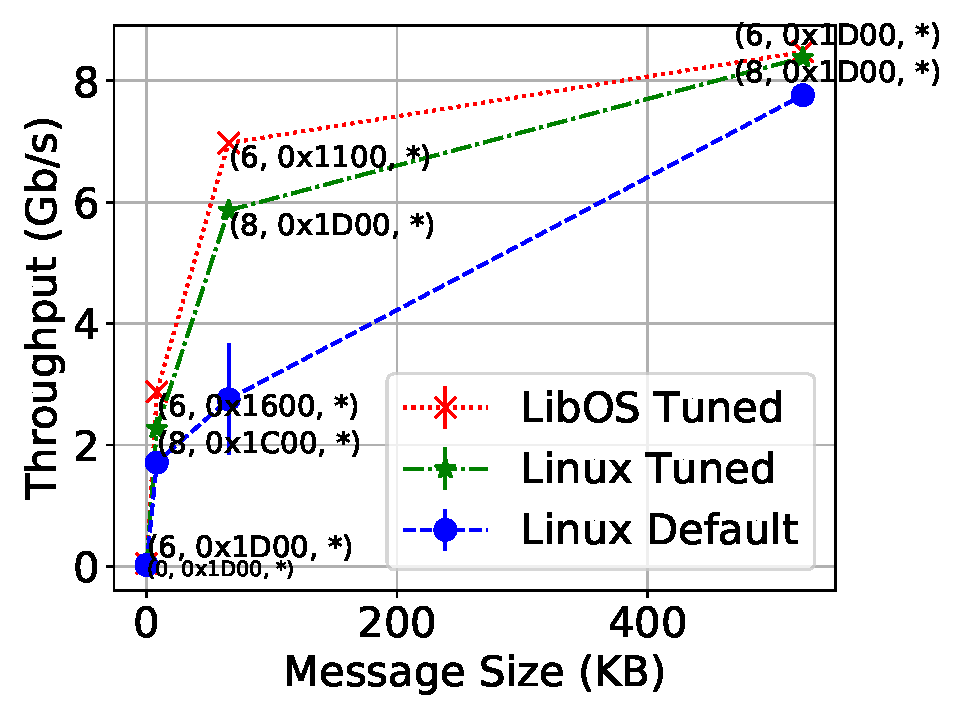
\includegraphics[width=1\textwidth]{osdi_figures/netpipe_tput}
        \end{subfigure}
 %      \hfill
        \begin{subfigure}[b]{0.32\textwidth}  
            \centering 
            \caption[]%
            {{\small Memcached}} 
            \vspace*{-0.3cm}    
            \label{fig:perf_mcd}
            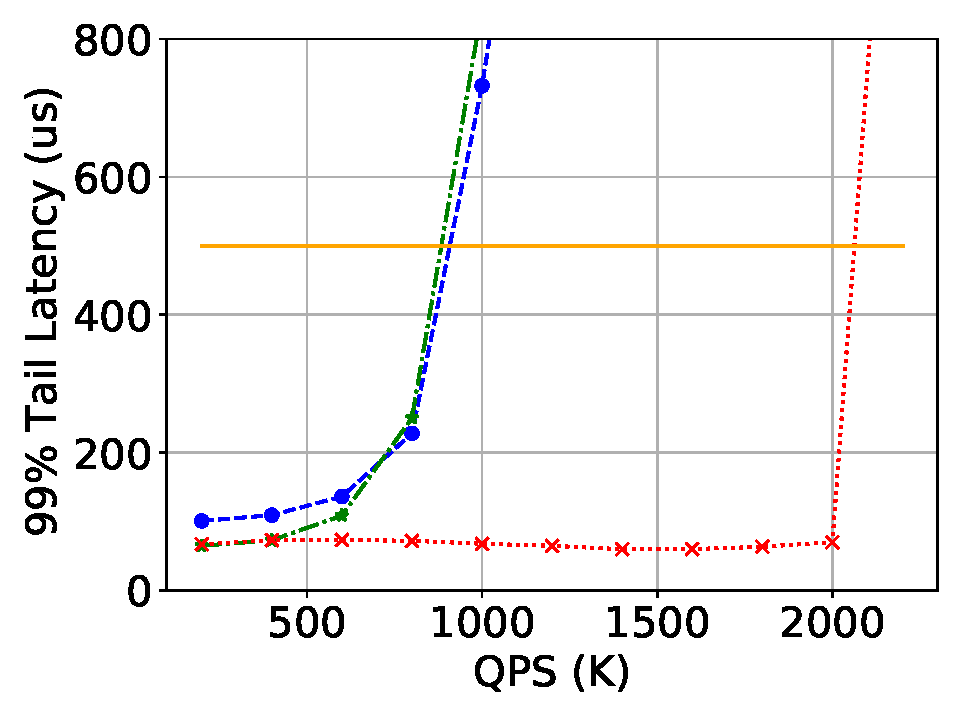
\includegraphics[width=1\textwidth]{osdi_figures/mcd_sla.pdf}
        \end{subfigure}
 %      \hfill
 %     \hspace{0.8cm}
        \begin{subfigure}[b]{0.32\textwidth}   
            \centering 
            \caption[]%
            {{\small Memcached-silo}} 
             \vspace*{-0.3cm}     
            \label{fig:perf_mcdsilo}
            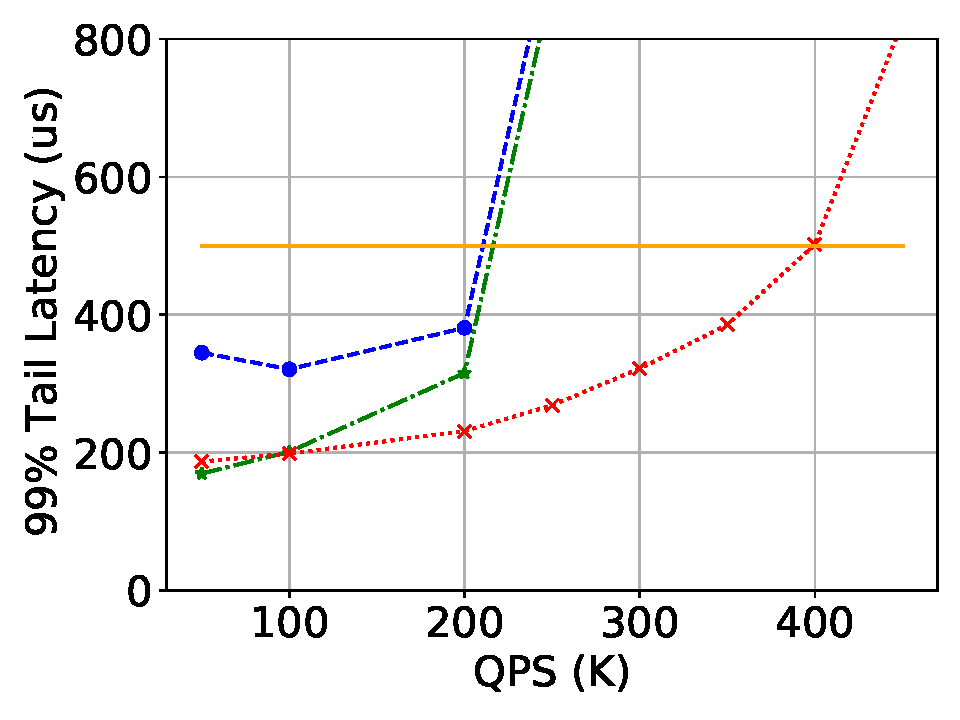
\includegraphics[width=1\textwidth]{osdi_figures/mcdsilo_sla.pdf}
        \end{subfigure}
        %\vspace*{0.3cm}  
        \caption[]
        {\small Performance baselines for NetPIPE across message sizes (64 B, 8 KB, 64 KB, and 512 KB) and  Memcached and Memcached-silo across different QPS rates.
For netpipe, the standard deviation around mean throughput is shown
for each message size.
The orange lines in both Memcached plots indicate an SLA objective of 500 {\micro}s.} 
        \label{fig:perf}
    \end{figure*}
